\documentclass[10pt,a4paper]{article}
% ===================== PAQUETES =====================
\usepackage[utf8]{inputenc}
\usepackage[T1]{fontenc}
\usepackage[spanish,es-tabla]{babel}
\usepackage{amsmath,amssymb}
\usepackage{geometry}
\usepackage{enumitem}
\usepackage{hyperref}
\usepackage{fancyhdr}
\usepackage{titlesec}
\usepackage{setspace}
\usepackage{graphicx}
\usepackage{caption}
\usepackage{xcolor}
\usepackage{float}
\usepackage{pgfplots}
\pgfplotsset{compat=1.18}
\usepackage{pdflscape}
\usepackage{tabularx}
\usepackage{array}
\usepackage{booktabs}

% ===================== CONFIGURACIÓN =====================
\geometry{margin=2.5cm}
\setstretch{1.15}
\hypersetup{
    colorlinks=true,
    linkcolor=black,
    urlcolor=blue
}

\pagestyle{fancy}
\fancyhf{}
\captionsetup{font=small}
\setlength{\headheight}{32pt}

% FECHA
\usepackage{datetime}
\newdateformat{monthyeardate}{%
  \monthname[\THEMONTH], \THEYEAR}

% Header
\lhead{
    
\includegraphics[width=3.6cm]{Logos/header_utfsm.png}
}
\rhead{
    
\includegraphics[width=1.3cm]{Logos/Logo_industrias.png}
}

% Footer
\newcommand{\theCampus}{Vitacura}
\lfoot{\footnotesize ICN-292 — Sistemas de Información para la Gestión}
\cfoot{\footnotesize \thepage}

% Líneas
\renewcommand{\headrulewidth}{0.4pt}
\renewcommand{\footrulewidth}{0.4pt}

\usepackage{setspace}

\setlength{\parindent}{0pt}
\setlength{\parskip}{2pt}
\usepackage{listings}
\setlength{\headheight}{40pt}

\lstdefinestyle{sqlLaboratorio}{
    basicstyle=\ttfamily\footnotesize,
    columns=fullflexible,
    keepspaces=true,
    showstringspaces=false,
    breaklines=true,
    frame=single,
    framerule=0.35pt,
    rulecolor=\color{black!40},
    backgroundcolor=\color{black!2},
    aboveskip=5pt,
    belowskip=7pt,
    xleftmargin=3pt,
    xrightmargin=3pt,
    literate={á}{{\'a}}1 {é}{{\'e}}1 {í}{{\'i}}1 {ó}{{\'o}}1 {ú}{{\'u}}1 {ñ}{{\~n}}1 {Á}{{\'A}}1 {É}{{\'E}}1 {Í}{{\'I}}1 {Ó}{{\'O}}1 {Ú}{{\'U}}1
}
\lstset{style=sqlLaboratorio}

\begin{document}
\begin{center}
\vspace{-2mm}
{\Huge Laboratorio 5 --- SQL (2/2)}\\
{\Large \sc{ICN-292 --- Sistemas de Información para la Gestión}}
\vspace{2mm}
\hrule
\textbf{Charles Piket Silva}\\
{\small Ingeniería Civil Industrial, 202360512-3, \emph{cpiket@usm.cl}}\\
{\small \textbf{Repositorio GitHub:} https://github.com/Cpikets/ICN292-Lab5-Piket-Charles}
\end{center}
\vspace{5mm}

\section*{Consulta 1}
\begin{lstlisting}
SELECT vd.nombre AS vendedor,
       COUNT(v.id_venta) AS cantidad_ventas
FROM vendedores AS vd
LEFT JOIN ventas AS v ON v.id_vendedor = vd.id_vendedor
GROUP BY vd.id_vendedor, vd.nombre
ORDER BY cantidad_ventas DESC, vd.nombre ASC;
\end{lstlisting}

\begin{figure}[H]
    \centering
    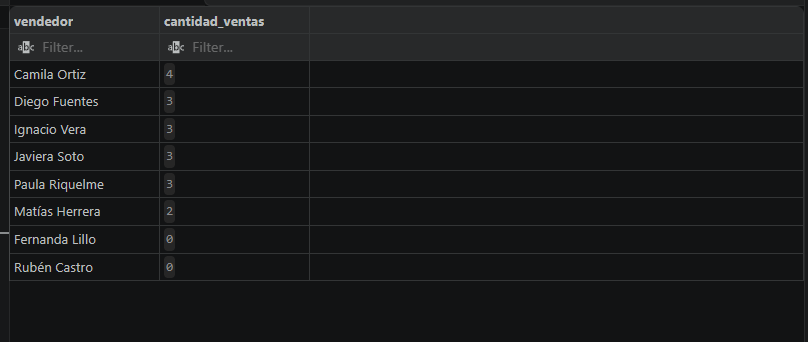
\includegraphics[width=0.97\linewidth,keepaspectratio]{Evidencia_lab5/Consulta_01.png}
    \caption{Vendedores y cantidad de ventas registradas; incluye quienes no vendieron.}
\end{figure}

\clearpage
\section*{Consulta 2}
\begin{lstlisting}
SELECT t.nombre AS tienda,
       COUNT(v.id_venta) AS cantidad_ventas,
       COALESCE(SUM(v.unidades), 0) AS unidades_vendidas
FROM tiendas AS t
LEFT JOIN vendedores AS vd ON vd.id_tienda = t.id_tienda
LEFT JOIN ventas AS v ON v.id_vendedor = vd.id_vendedor
GROUP BY t.id_tienda, t.nombre
ORDER BY unidades_vendidas DESC, t.nombre ASC;
\end{lstlisting}

\begin{figure}[H]
    \centering
    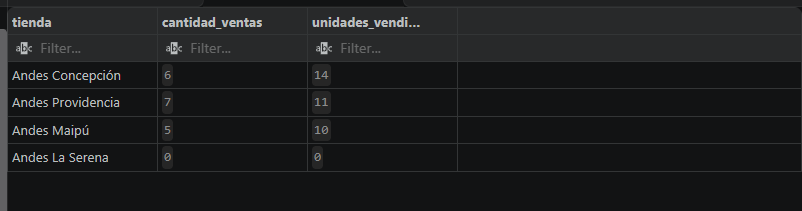
\includegraphics[width=0.97\linewidth,keepaspectratio]{Evidencia_lab5/Consulta_02.png}
    \caption{Ventas y unidades por tienda, incluida Andes La Serena con cero ventas.}
\end{figure}

\section*{Consulta 3}
\begin{lstlisting}
SELECT t.nombre AS tienda,
       t.comuna
FROM tiendas AS t
LEFT JOIN vendedores AS vd ON vd.id_tienda = t.id_tienda
WHERE vd.id_vendedor IS NULL
ORDER BY t.nombre ASC;
\end{lstlisting}

\begin{figure}[H]
    \centering
    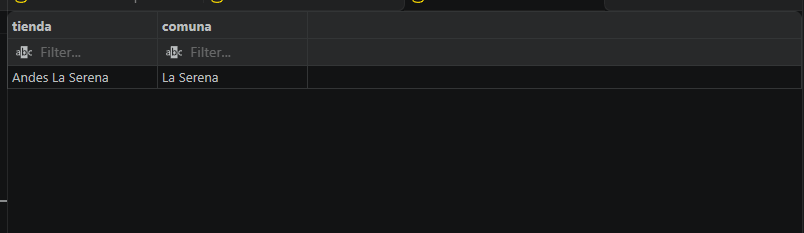
\includegraphics[width=0.97\linewidth,keepaspectratio]{Evidencia_lab5/Consulta_03.png}
    \caption{Tienda que no tiene vendedores asignados.}
\end{figure}

\clearpage
\section*{Consulta 4}
\begin{lstlisting}
SELECT b.modelo, b.categoria
FROM bicicletas AS b
LEFT JOIN ventas AS v
    ON v.id_bicicleta = b.id_bicicleta
   AND v.fecha >= '2025-06-01'
   AND v.fecha < '2025-07-01'
WHERE v.id_venta IS NULL
ORDER BY b.modelo ASC;
\end{lstlisting}

El mes se filtró en el \texttt{ON}; en el \texttt{WHERE} se eliminarían las filas sin ventas en junio.

\begin{figure}[H]
    \centering
    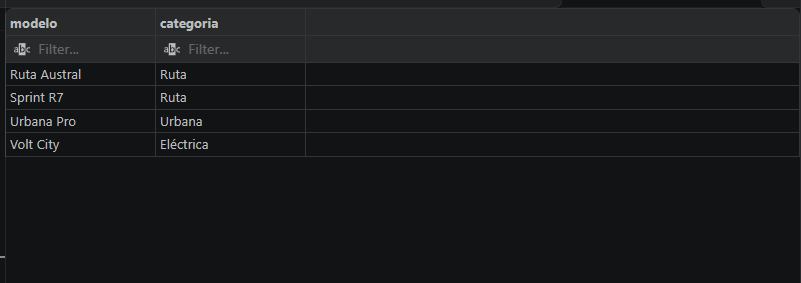
\includegraphics[width=0.97\linewidth,keepaspectratio]{Evidencia_lab5/Consulta_04.png}
    \caption{Modelos que no registraron ventas durante junio de 2025.}
\end{figure}

\section*{Consulta 5}
\begin{lstlisting}
SELECT vd.nombre AS vendedor,
       COALESCE(t.nombre, 'Sin tienda asignada') AS tienda
FROM vendedores AS vd
LEFT JOIN tiendas AS t ON t.id_tienda = vd.id_tienda
WHERE NOT EXISTS (
    SELECT 1
    FROM ventas AS v
    WHERE v.id_vendedor = vd.id_vendedor
)
ORDER BY vd.nombre ASC;
\end{lstlisting}

\begin{figure}[H]
    \centering
    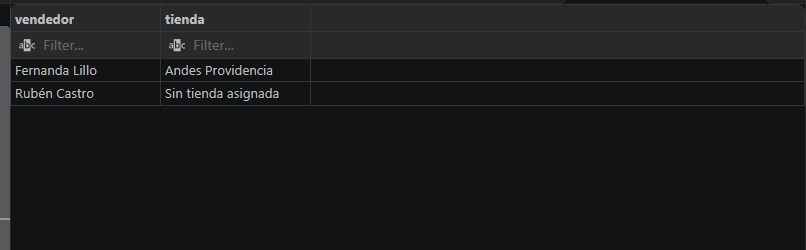
\includegraphics[width=0.97\linewidth,keepaspectratio]{Evidencia_lab5/Consulta_05.png}
    \caption{Vendedores sin ventas y sus tiendas, incluida la ausencia de asignación.}
\end{figure}

\clearpage
\section*{Consulta 6}
\begin{lstlisting}
SELECT v1.nombre AS vendedor_primero,
       v2.nombre AS vendedor_despues,
       v1.fecha_ingreso AS fecha_primero,
       v2.fecha_ingreso AS fecha_despues,
       t.nombre AS tienda
FROM vendedores AS v1
INNER JOIN vendedores AS v2
    ON v1.id_tienda = v2.id_tienda
   AND v1.fecha_ingreso < v2.fecha_ingreso
INNER JOIN tiendas AS t ON t.id_tienda = v1.id_tienda
ORDER BY t.nombre ASC, v1.fecha_ingreso ASC,
         v2.fecha_ingreso ASC, v1.nombre ASC, v2.nombre ASC;
\end{lstlisting}

\begin{figure}[H]
    \centering
    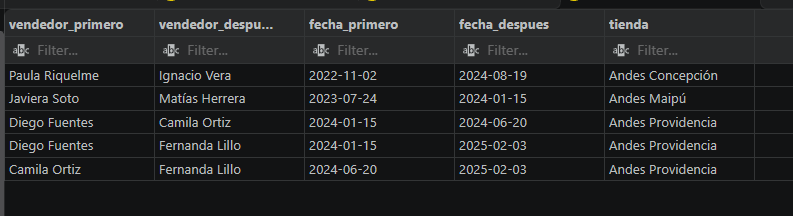
\includegraphics[width=0.97\linewidth,keepaspectratio]{Evidencia_lab5/Consulta_06.png}
    \caption{Pares de vendedores de una misma tienda, ordenados por fecha de ingreso.}
\end{figure}


\section*{Consulta 7}
\begin{lstlisting}
SELECT t.nombre AS tienda,
       SUM(v.unidades * b.precio) AS monto_montana_ruta
FROM tiendas AS t
INNER JOIN vendedores AS vd ON vd.id_tienda = t.id_tienda
INNER JOIN ventas AS v ON v.id_vendedor = vd.id_vendedor
INNER JOIN bicicletas AS b ON b.id_bicicleta = v.id_bicicleta
WHERE b.categoria IN ('Montaña', 'Ruta')
GROUP BY t.id_tienda, t.nombre
HAVING SUM(v.unidades * b.precio) > 2000000
ORDER BY monto_montana_ruta DESC, t.nombre ASC;
\end{lstlisting}

\begin{figure}[H]
    \centering
    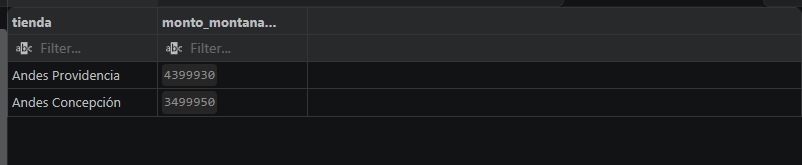
\includegraphics[width=0.97\linewidth,keepaspectratio]{Evidencia_lab5/Consulta_07.png}
    \caption{Tiendas con más de dos millones vendidos en las categorías Montaña y Ruta.}
\end{figure}

\newpage
\section*{Consulta 8}
\begin{lstlisting}
SELECT b.modelo,
       b.precio
FROM bicicletas AS b
WHERE b.precio > (
    SELECT AVG(b2.precio)
    FROM bicicletas AS b2
)
ORDER BY b.precio DESC, b.modelo ASC;
\end{lstlisting}

El promedio se obtuvo con \texttt{AVG(precio)} sobre los ocho modelos de \texttt{bicicletas}; el valor es \$657.490.

\begin{figure}[H]
    \centering
    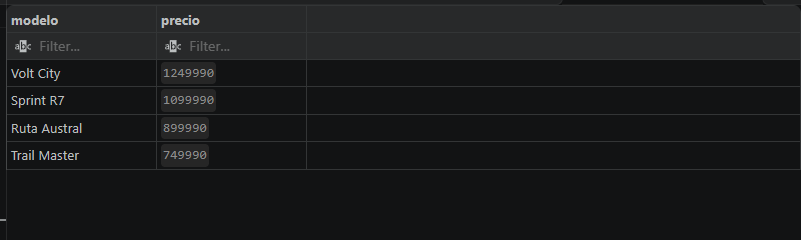
\includegraphics[width=0.97\linewidth,keepaspectratio]{Evidencia_lab5/Consulta_08.png}
    \caption{Modelos cuyo precio supera el promedio del catálogo.}
\end{figure}


\section*{Consulta 9}
\begin{lstlisting}
SELECT vd.nombre AS vendedor,
       ROUND(AVG(v.unidades), 2) AS promedio_unidades_por_venta
FROM vendedores AS vd
INNER JOIN ventas AS v ON v.id_vendedor = vd.id_vendedor
GROUP BY vd.id_vendedor, vd.nombre
HAVING AVG(v.unidades) > (
    SELECT AVG(v2.unidades)
    FROM ventas AS v2
)
ORDER BY promedio_unidades_por_venta DESC, vd.nombre ASC;
\end{lstlisting}

\begin{figure}[H]
    \centering
    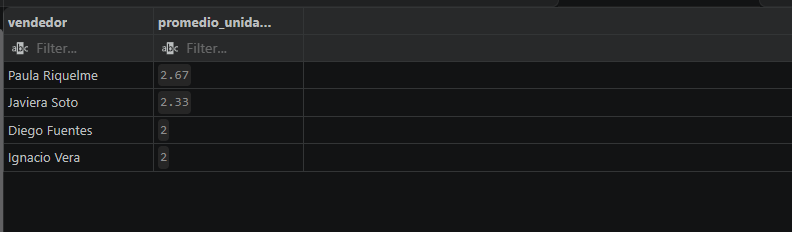
\includegraphics[width=0.97\linewidth,keepaspectratio]{Evidencia_lab5/Consulta_09.png}
    \caption{Vendedores con promedio de unidades por venta superior al promedio general.}
\end{figure}

\newpage
\section*{Consulta 10}
\begin{lstlisting}
SELECT vd.nombre AS vendedor,
       COALESCE(SUM(v.unidades * b.precio), 0) AS monto_total_vendido
FROM vendedores AS vd
LEFT JOIN ventas AS v ON v.id_vendedor = vd.id_vendedor
LEFT JOIN bicicletas AS b ON b.id_bicicleta = v.id_bicicleta
GROUP BY vd.id_vendedor, vd.nombre
ORDER BY monto_total_vendido DESC, vd.nombre ASC;
\end{lstlisting}

El \texttt{INNER JOIN} excluye a los que no vendieron; con \texttt{LEFT JOIN} y \texttt{COALESCE} aparecen con cero.

\begin{figure}[H]
    \centering
    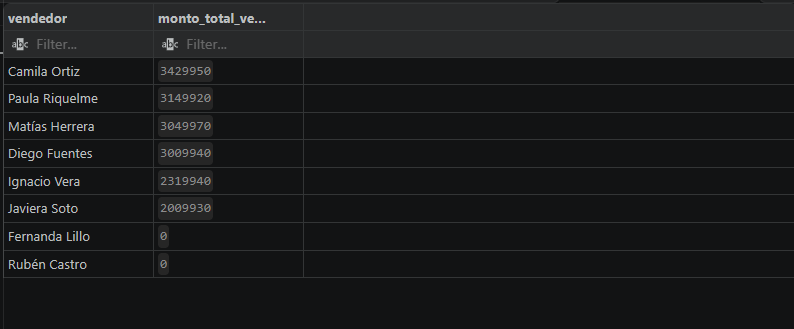
\includegraphics[width=0.97\linewidth,keepaspectratio]{Evidencia_lab5/Consulta_10.png}
    \caption{Monto vendido por cada vendedor, incluidos quienes registran cero.}
\end{figure}

\end{document}
